\section{Layout delle tabelle}
\begin{frame}[fragile]
 \frametitle{Layout delle tabelle}

 Gli elementi della tabella possono essere modificati per ottenere migliorare l'estetica del documento.
 \begin{itemize}
     \item con il comando \inline{\setlength{\arrayrulewidth}{1mm}} si pu\`o impostare lo spessore dei bordi della tabella
     \item con il comando \inline{\setlength{\tabcolsep}{18pt}} si pu\`o impostare lo spazio tra il testo e il bordo sinistro/destro della cella
     \item il comando \inline{\renewcommand{\arraystretch}{1.5}} imposta l'altezza di ogni riga
 \end{itemize}
\end{frame}

\begin{frame}
 \frametitle{Colorare le righe - 1}
 È prassi comune utilizzare due colori per alternare le righe in una tabella per migliorare la leggibilità. Questo può essere ottenuto in \LaTeX con il pacchetto xcolor: \\ \inline{\usepackage[table]{xcolor}} \\
 e poi utilizzando il comando:\\
 \inline{\rowcolors{3}{colore_1}{colore_2}}
 \end{frame}
 
 \begin{frame}
 \frametitle{Colorare le righe - 2}
 \begin{esempio}{Righe Colorate}
    \begin{code}
        \inputminted[linenos, fontsize=\footnotesize] {latex} {res/examples/tabellaColorata.tex}
    \end{code}
 \end{esempio}
\end{frame}

\begin{frame}
 \frametitle{Colorare le righe - 3}
  Il risultato \`e il seguente:
   \centering
   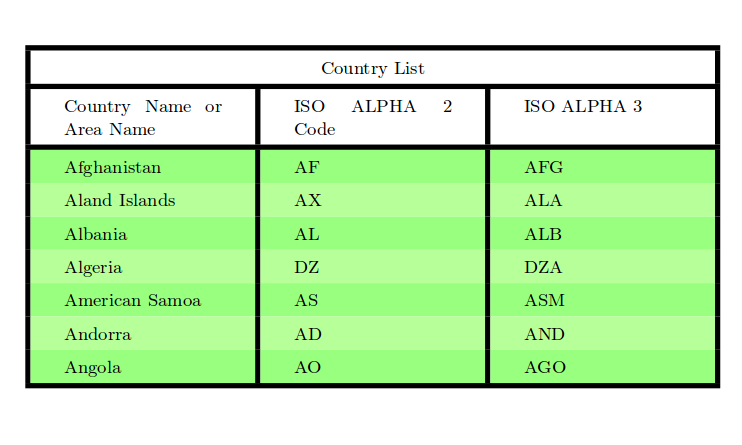
\includegraphics[scale=0.4]{res/images/TablesColored}
\end{frame}